\documentclass[tikz,border=6pt]{standalone}
\usepackage{helvet}
\renewcommand{\familydefault}{\sfdefault}
\begin{document}
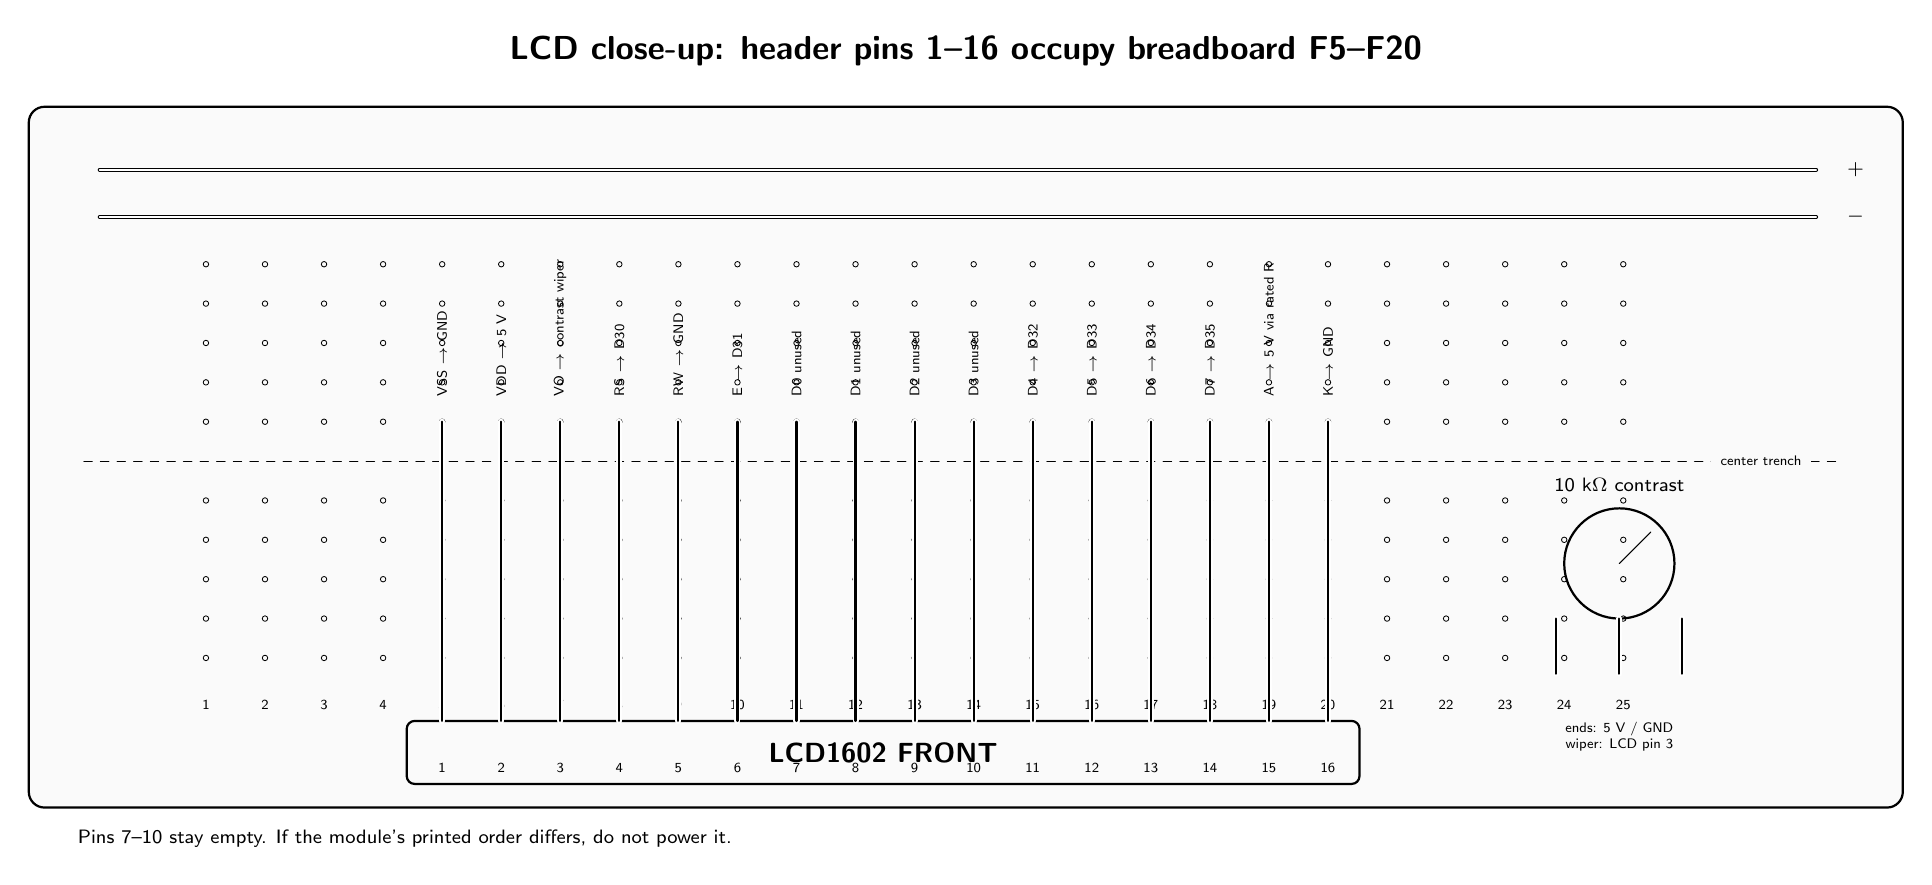
\begin{tikzpicture}[x=1mm,y=1mm,line cap=round,line join=round,
  hole/.style={circle,draw,line width=.3pt,inner sep=.7pt},
  wire/.style={preaction={draw=white,line width=2.2pt},line width=.8pt},
  tiny/.style={font=\fontsize{5.2}{5.8}\selectfont},
  small/.style={font=\scriptsize}]
\node[font=\bfseries\large] at (124,103)
  {LCD close-up: header pins 1--16 occupy breadboard F5--F20};
\draw[rounded corners=2mm,line width=.8pt,fill=black!2] (5,7) rectangle (243,96);
\draw[double] (14,88)--(232,88);\node[small] at (237,88) {$+$};
\draw[double] (14,82)--(232,82);\node[small] at (237,82) {$-$};
\foreach \r in {1,...,25}
{
  \pgfmathsetmacro{\xx}{20+\r*7.5}
  \foreach \yy in {26,31,36,41,46,56,61,66,71,76}
    \node[hole] at (\xx,\yy) {};
  \node[tiny] at (\xx,20) {\r};
}
\draw[dashed] (12,51)--(235,51);
\node[tiny,fill=black!2] at (225,51) {center trench};
\draw[rounded corners=1mm,line width=.8pt] (53,10) rectangle (174,18);
\node[small,font=\bfseries] at (113.5,14) {LCD1602 FRONT};
\foreach \n in {1,...,16}
{
  \pgfmathsetmacro{\xx}{50+\n*7.5}
  \draw[wire] (\xx,18)--(\xx,56);
  \node[tiny] at (\xx,12) {\n};
}
\node[tiny,rotate=90,anchor=west] at (57.5,58) {VSS $\to$ GND};
\node[tiny,rotate=90,anchor=west] at (65,58) {VDD $\to$ 5 V};
\node[tiny,rotate=90,anchor=west] at (72.5,58) {VO $\to$ contrast wiper};
\node[tiny,rotate=90,anchor=west] at (80,58) {RS $\to$ D30};
\node[tiny,rotate=90,anchor=west] at (87.5,58) {RW $\to$ GND};
\node[tiny,rotate=90,anchor=west] at (95,58) {E $\to$ D31};
\node[tiny,rotate=90,anchor=west] at (102.5,58) {D0 unused};
\node[tiny,rotate=90,anchor=west] at (110,58) {D1 unused};
\node[tiny,rotate=90,anchor=west] at (117.5,58) {D2 unused};
\node[tiny,rotate=90,anchor=west] at (125,58) {D3 unused};
\node[tiny,rotate=90,anchor=west] at (132.5,58) {D4 $\to$ D32};
\node[tiny,rotate=90,anchor=west] at (140,58) {D5 $\to$ D33};
\node[tiny,rotate=90,anchor=west] at (147.5,58) {D6 $\to$ D34};
\node[tiny,rotate=90,anchor=west] at (155,58) {D7 $\to$ D35};
\node[tiny,rotate=90,anchor=west] at (162.5,58) {A $\to$ 5 V via rated R};
\node[tiny,rotate=90,anchor=west] at (170,58) {K $\to$ GND};
\draw[line width=.8pt] (207,38) circle (7);
\draw (207,38)--(211,42);
\draw[wire] (199,31)--(199,24);
\draw[wire] (207,31)--(207,24);
\draw[wire] (215,31)--(215,24);
\node[small] at (207,48) {10 k$\Omega$ contrast};
\node[tiny,align=center] at (207,16)
  {ends: 5 V / GND\\wiper: LCD pin 3};
\node[small,anchor=west] at (10,3)
  {Pins 7--10 stay empty. If the module's printed order differs, do not power it.};
\end{tikzpicture}
\end{document}
